\chapter{Embodiment Design}
The next phase in the design methodology is embodiment design. This phase, as defined by Pahl and Beitz \cite{Pahl07t}, involves starting with the fundamental solution or concept for a technical product and then advancing the design in alignment with technical and economic criteria, taking into account further information. The ultimate objective is to reach a stage where the subsequent detailed design can smoothly progress into the production phase.
Figure \ref{fig:embodiment_design} shows the steps involved in this phase.

\begin{figure}
    \centering
    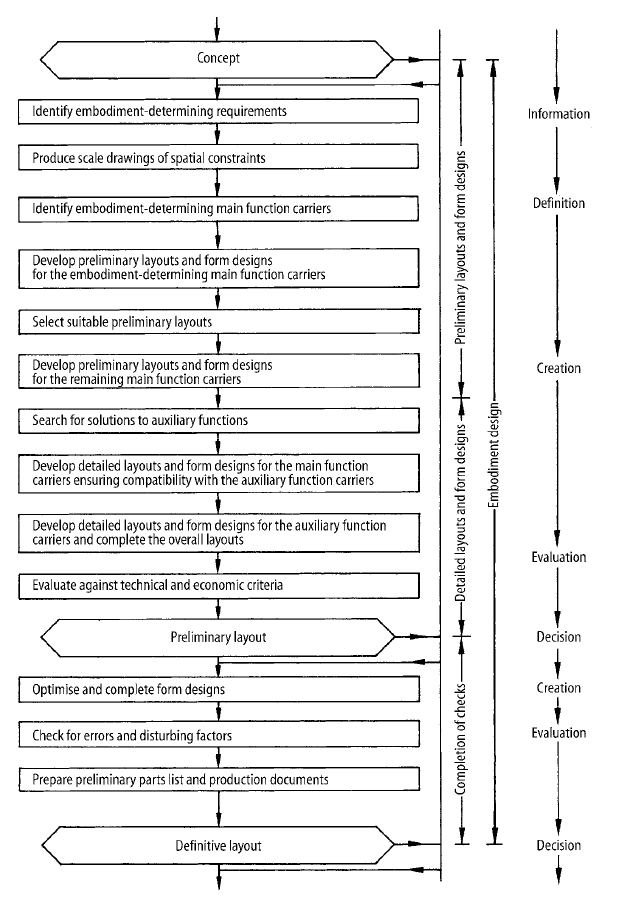
\includegraphics[width=0.92\linewidth]{texs/Part1/chapter4/image/embodiment.png}
    \caption{Steps in Embodiment Design \cite{Pahl07u}}
    \label{fig:embodiment_design}
\end{figure}

\section{Basic Rules of Embodiment Design}
When it comes to product design, there are some basic rules that must be followed. As defined by Pahl and Beitz \cite{Pahl07v}, they include clarity, simplicity, and safety. Neglecting these rules can potentially result in issues and accidents. Subsequent sections will provide a comprehensive exploration of these guidelines.

\subsection{Clarity}
Clarity, as described by Pahl and Beitz \cite{Pahl07w}, entails establishing clear and unambiguous connections within a design. This involves ensuring straightforward relationships between subfunctions, inputs, and outputs to prevent any confusion or misinterpretation. It also extends to the selection of a working principle, where designers should choose principles that clarify cause-and-effect dynamics, align with the product's purpose, and optimize its layout by eliminating unnecessary complexity.

Additionally, clarity applies to the broader design structure, whether it involves multiple working principles or component combinations. It mandates that the design facilitates the orderly flow of energy, materials, and signals, preventing adverse effects like excessive forces or wear. This commitment to clarity ultimately enhances the product's reliability and durability.

\subsection{Simplicity}
Simplicity \cite{Pahl07x} in design is epitomized by an uncomplicated and easily comprehensible approach, often achievable by using fewer components. Such simplicity can lead to cost savings, reduced wear and tear, and minimized maintenance requirements. Nonetheless, it's crucial to strike a balance, as certain functions inherently demand a minimum number of components.

Designers should, therefore, strive for a minimalist approach by employing the fewest components possible while maintaining straightforward shapes, as this promotes efficiency and practicality in the design process. The choice between numerous components with simple shapes, albeit potentially increasing production effort, and a single, more affordable cast component should be made while considering the specific problem and constraints.

\subsection{Safety}
Safety \cite{Pahl07y} considerations are crucial in ensuring both the effective performance of technical functions and the protection of people and the environment. Designers rely on a safety methodology outlined in the German industry standard DIN 31 000, which encompasses three levels: direct safety, indirect safety, and warnings. In general, designers should prioritize direct safety measures, seeking solutions that inherently eliminate potential dangers. Only when this is not feasible should they resort to indirect safety measures, involving the construction of specialized protective systems.

Warnings, which serve to highlight dangers and hazard zones, are best utilized in conjunction with direct and indirect safety measures, clarifying specific risks. As designers address technical challenges, they encounter various constraints, not all of which can be simultaneously overcome. However, their objective remains to develop solutions that come as close as possible to meeting all requirements. It's important to note that exceptionally high safety demands can complicate design, potentially diminishing clarity and economic viability, and even leading to project abandonment in some cases.

\section{Guideline of Embodiment Design}
In addition the the basic rules of embodiment design, Pahl and Beitz \cite{Pahl07z} also stress the importance of following a set of design guidelines to help designers meet the specific requirements and constraints. For this project, the following design guidelines are considered:

\begin{itemize}
    \item Design for production
    \item Design for ergonomics
\end{itemize}

\subsection{Design for Production}
Design for production \cite{Pahl07aa} is a design guideline that emphasizes the importance of considering the production process during the design phase. This approach enables designers to optimize the production cost and times while ensuring the product's functionality and quality. By following the basic rules of clarity and simplicity, designers are already on the right track to achieving this goal.

\subsubsection{Appropriate Overall Layout Design}
Overall layout design, derived from the function structure, influences product division into assemblies and components, including sourcing decisions (in-house, bought-out, standard parts), production procedures, dimensions, batch sizes, joining methods, and quality control.

The layout can lead to differential, integral, composite, or building-block construction methods. Differential Construction involves breaking down components into easily produced parts, facilitating adaptability, increased component batch sizes, and easier quality assurance. However, it demands greater machining and assembly costs and may have functional limitations due to joints.

Integral Construction combines multiple parts into a single component, reducing costs due to integration but can be complex and sensitive to market conditions. Composite Construction involves connecting different parts requiring further work, applying multiple joining methods or using various materials for optimal property utilization.

Building Block Construction results from splitting components so that the parts or assemblies can be used in other products or variants, offering flexibility and cost savings. These construction methods offer specific advantages and disadvantages, depending on the context and design requirements.

\subsubsection{Appropriate Form Design of Components}
During component form design, designers significantly impact production costs, times, and product quality by choosing shapes, dimensions, surface finishes, tolerances, and fits. These choices influence production procedures, machine types, in-house vs. bought-out components, materials, and quality control procedures.

Conversely, production facilities influence design features, which may include dimension limitations necessitating component division or the acquisition of bought-out components. Many guidelines exist for appropriate component form design, and tolerances are crucial.
Figure \ref{fig:guideline} shows the design guidelines for designing components specifically for 3D printing.

\begin{figure}
    \centering
    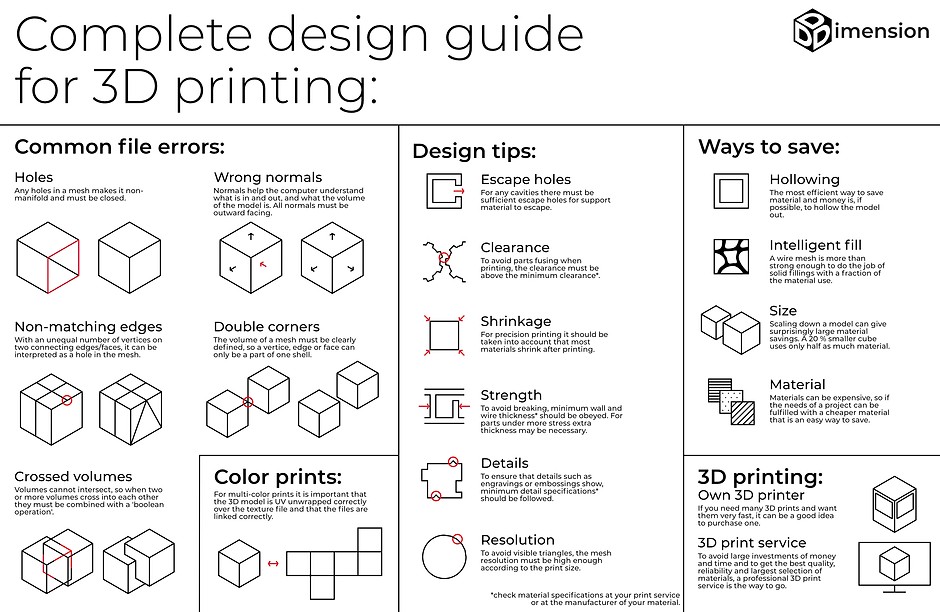
\includegraphics[width=0.92\linewidth]{texs/Part1/chapter4/image/guidelines.png}
    \caption{Design guidelines for 3D printing \cite{DDDimension_22}}
    \label{fig:guideline}
\end{figure}

\subsection{Design for Ergonomics}
Ergonomics \cite{Pahl07ab} is vital in designing technical products, aiming to align them with human characteristics, needs, and interfaces. It covers a broad range of items, including everyday household products and human-machine interfaces. Recent focus has shifted to user-friendly interfaces and ergonomic workplace assessment tools.

Ergonomic design considers various factors, starting with biomechanics, which addresses how body postures and movements interact with product design. Physiological aspects, such as muscle action, circulation, and temperature regulation, are crucial. Sensory factors like light and noise must also be taken into account. Psychological aspects guide design to minimize cognitive load and enhance user-friendliness.

Ergonomics extends to active and passive user involvement. Active involvement necessitates careful planning, assessing if human interaction is necessary and effective. Passive involvement addresses how users are affected by products, considering factors like energy flows, vibrations, light, climate, and noise.

Identifying ergonomic requirements can follow two approaches. The object-based approach is used when designing predefined systems or products, employing checklists tailored to specific items. The effect-based approach applies to new situations, analyzing the effects of energy, material, and signal flows, ensuring they meet ergonomic requirements. Both aim to prioritize user comfort, safety, and efficiency while minimizing discomfort and errors.

\section{Preliminary Design}
In this section, we will explore multiple designs for the device. These designs are detailed 3D models of the device that we will use to evaluate their respective designs and assess their feasibility. Each of these preliminary designs will be based on the selected solution from the previous phase. Alongside the models, we will also present the production costs for each of these designs. For a more detailed breakdown of the production costs, please refer to Appendix \ref{appendix:production_cost}.


\subsection{Preliminary Design Variant 2}
\label{subsec:preliminary_design_variant_2}
In this section, we present a comprehensive design overview of Solution Variant 2. Figure \ref{fig:preliminary_design_variant_2} showcases the 3D model of Variant 2, while Figure \ref{fig:variant2_views} provides various perspectives and body measurements of the device. The key emphasis of this design is its ergonomic shape and user-friendly attributes. With a thickness of 49.2 mm (Figure \ref{fig:variant2_right_view}), it successfully strikes a balance between being slim and accommodating essential components for optimal performance.

\begin{figure}[h!]
    \centering
    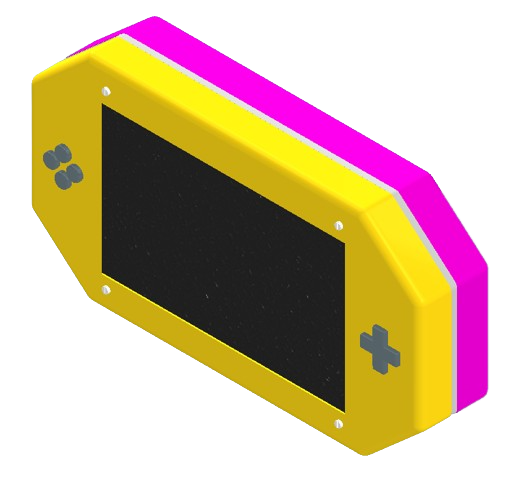
\includegraphics[height=5 cm]{texs/Part1/chapter4/image/v21.png}
    \caption{Preliminary Design Variant 2}
    \label{fig:preliminary_design_variant_2}
\end{figure}

\begin{figure}[h!]
    \centering
    \begin{subfigure}[c]{0.65\textwidth}
        \begin{minipage}{\textwidth}
            \centering
            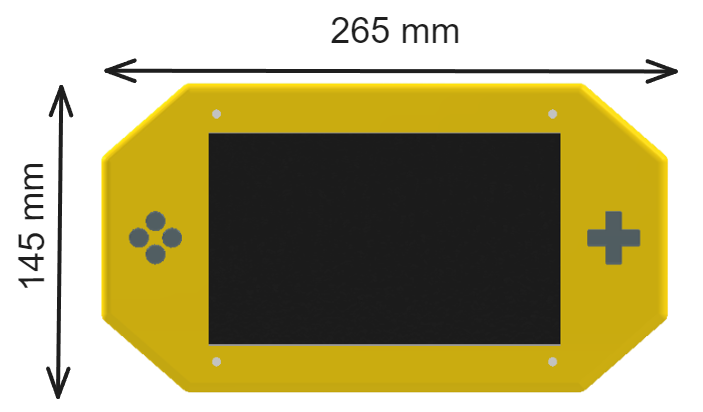
\includegraphics[height=4 cm]{texs/Part1/chapter4/image/v22.png}
        \end{minipage}
        \caption{Front View}
        \label{fig:variant2_front_view}
    \end{subfigure}
    % \hfill
    \begin{subfigure}[c]{0.25\textwidth}
        \begin{minipage}{\textwidth}
            \centering
            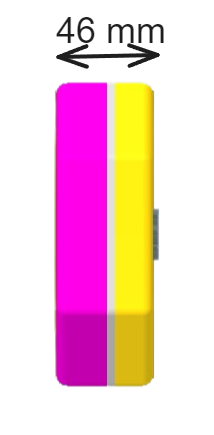
\includegraphics[height=4 cm]{texs/Part1/chapter4/image/v23.png}
        \end{minipage}
        \caption{Right View}
        \label{fig:variant2_right_view}
    \end{subfigure}
    \caption{Views of Preliminary Design Variant 2}
    \label{fig:variant2_views}
\end{figure}

\begin{figure}[h!]
    \centering
    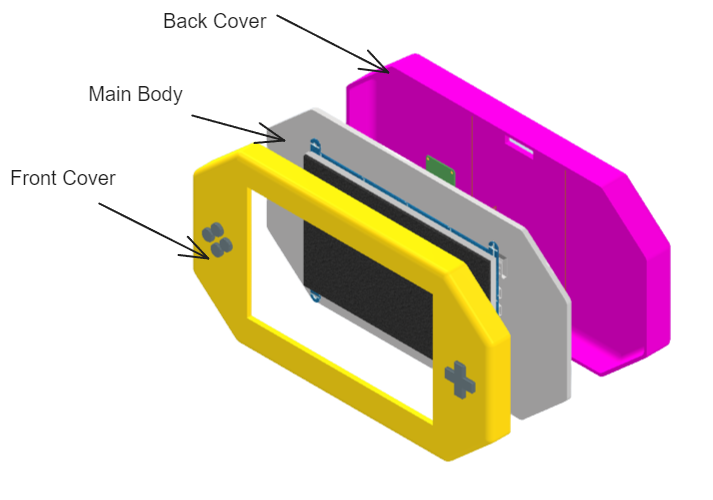
\includegraphics[width=0.5\linewidth]{texs/Part1/chapter4/image/v24.png}
    \caption{Body Components of Preliminary Design Variant 2}
    \label{fig:variant2_body_components}
\end{figure}

\begin{figure}[h!]
    \centering
    \begin{subfigure}[c]{0.5\textwidth}
        \begin{minipage}{\textwidth}
            \centering
            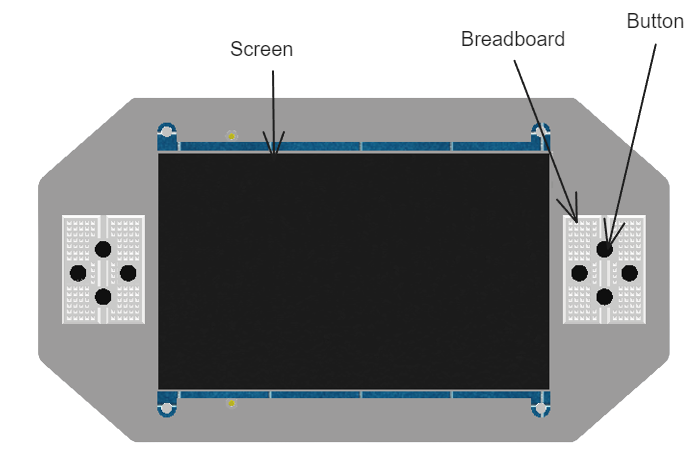
\includegraphics[height=4 cm]{texs/Part1/chapter4/image/v25.png}
        \end{minipage}
        \caption{Front View}
        \label{fig:variant2_front_view_main}
    \end{subfigure}
    % \hfill
    \begin{subfigure}[c]{0.5\textwidth}
        \begin{minipage}{\textwidth}
            \centering
            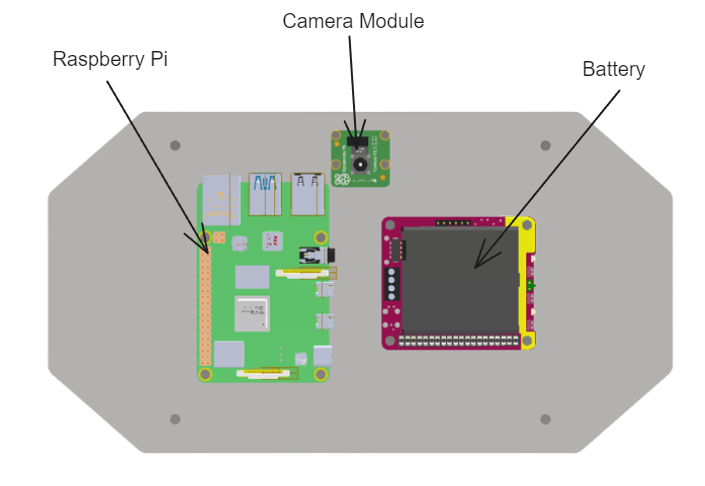
\includegraphics[height=4 cm]{texs/Part1/chapter4/image/v26.png}
        \end{minipage}
        \caption{Back View}
        \label{fig:variant2_back_view_main}
    \end{subfigure}
    \caption{Placement of inner components for Variant 2}
    \label{fig:variant2_inner_components}
\end{figure}

The physical design of Solution Variant 2 adheres to a sandwich-like structure comprising a main body, top cover, and back cover (Figure \ref{fig:variant2_body_components}). This design choice not only ensures the protection of internal components, but also simplifies assembly and maintenance. The main body of the device functions as the central hub, accommodating the internal components and features, whereas the top and back covers act as protective shields, safeguarding the internal parts from any damage that may result from external factors.

A crucial aspect of the design involves the arrangement of internal components within the device. Following a tablet-like configuration, the main LCD is positioned on the front side of the main body, providing users with a clear and interactive interface (Figure \ref{fig:variant2_front_view_main}). Simultaneously, the camera, Raspberry Pi, and battery were strategically placed on the back side of the body (Figure \ref{fig:variant2_back_view_main}) to optimize the weight distribution and ensure a well-balanced user experience. This arrangement enhances the overall usability and convenience of the device, making it suitable for a wide range of applications.

\begin{figure}[ht!]
    \centering
    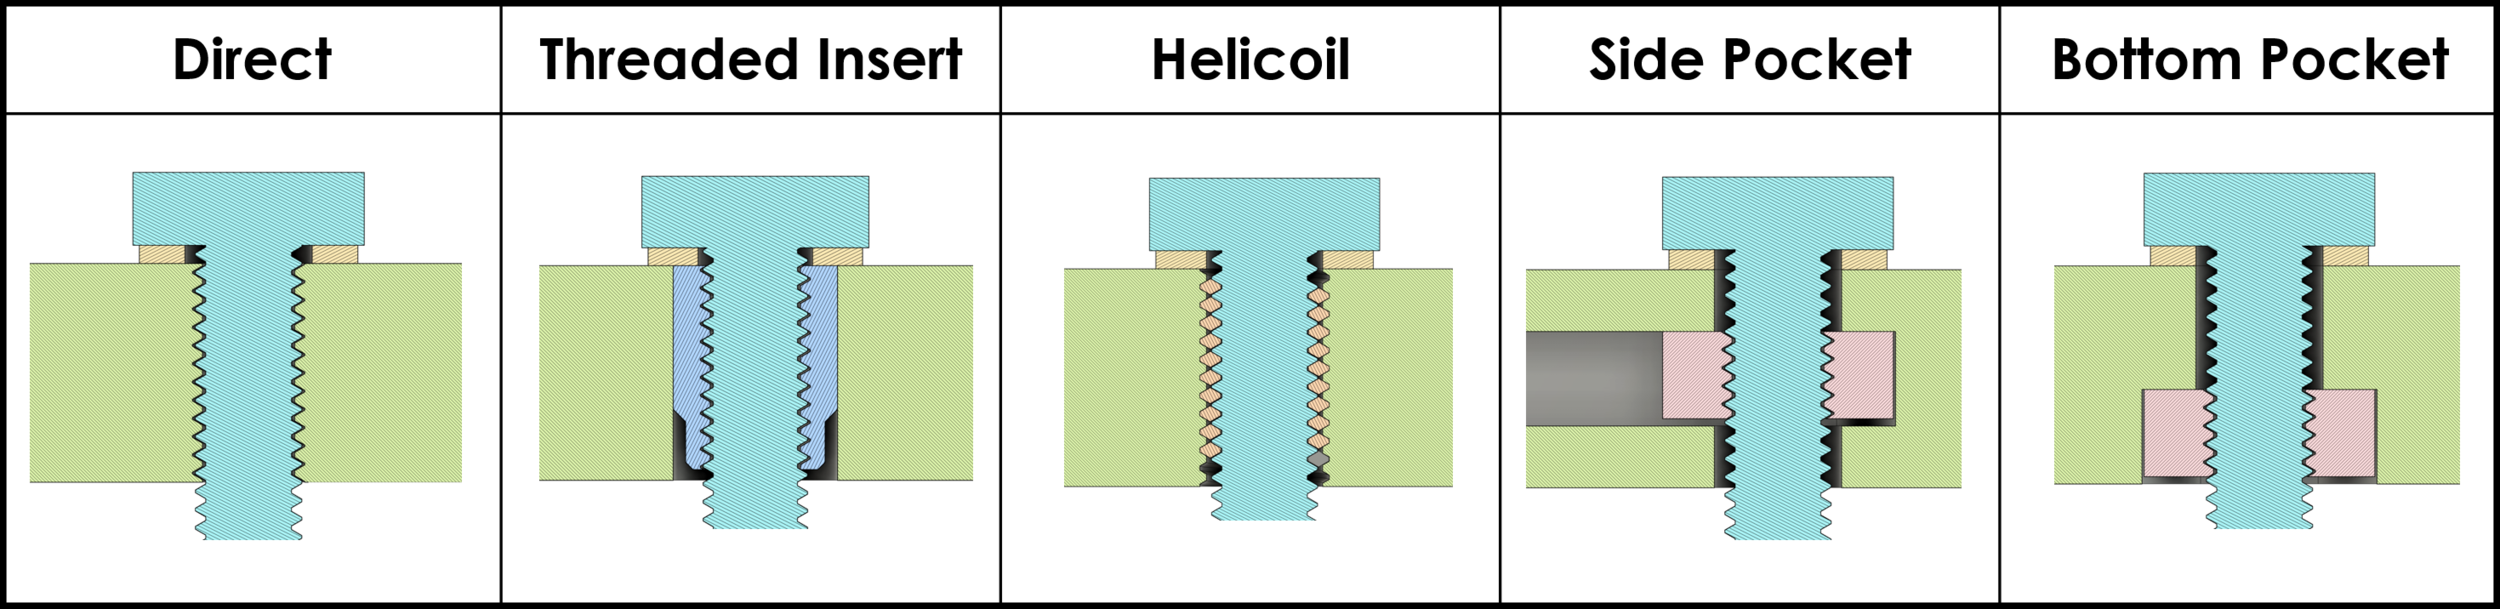
\includegraphics[width=\linewidth]{texs/Part1/chapter4/image/insert.png}
    \caption{Methods to secure components \cite{Hermann20}}
    \label{fig:insert}
\end{figure}

Ensuring the secure attachment of internal components to the main body is of primary importance in the design process. Various methods of component fastening have been considered, including direct attachment, threaded inserts, helicoils, side pockets, and bottom pockets, as shown in Figure \ref{fig:insert}.

The simplest approach is direct attachment, in which threads are designed into a 3D printed part to allow components to be screwed in. For more robust connections, threaded inserts can be used by designing holes in the 3D printed part and installing inserts appropriately.

Helicoils offer durable threaded holes by inserting coil-shaped inserts into the holes. Side pockets and bottom pockets involve creating cavities or slots in the 3D printed part to hold components securely. Each method has its own advantages and challenges. After careful evaluation, the variant opts for the use of threaded inserts due to its simplicity and robustness.

The battery, which is a critical component of the device, requires special attention to prevent any undesirable movement or instability. To address this concern, an effective method for firmly securing the battery in place is implemented by utilizing a battery cover. Figure \ref{fig:variant2_battery_cover} illustrates the design of the battery cover. The battery cover is then securely attached using screws and standoffs, ensuring that the battery remains in its designated position, even during vigorous handling or movement. Figure \ref{fig:variant2_battery_placement} shows the method used to secure the battery to the main body.

\begin{figure}[h!]
    \centering
    \begin{subfigure}[c]{\textwidth}
        \begin{minipage}{\textwidth}
            \centering
            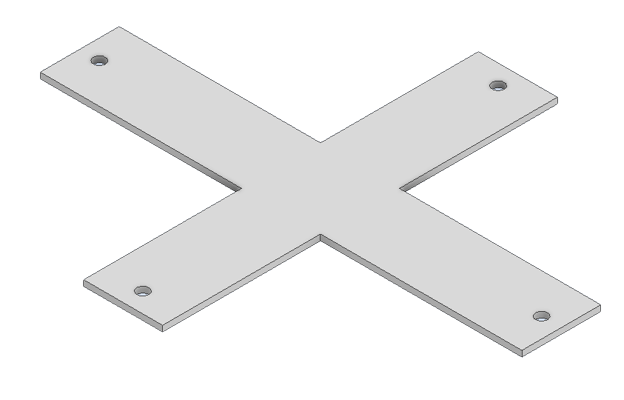
\includegraphics[height=4 cm]{texs/Part1/chapter4/image/v27.png}
        \end{minipage}
        \caption{Battery Cover}
        \label{fig:variant2_battery_cover}
    \end{subfigure}
    % \hfill
    \begin{subfigure}[c]{\textwidth}
        \begin{minipage}{\textwidth}
            \centering
            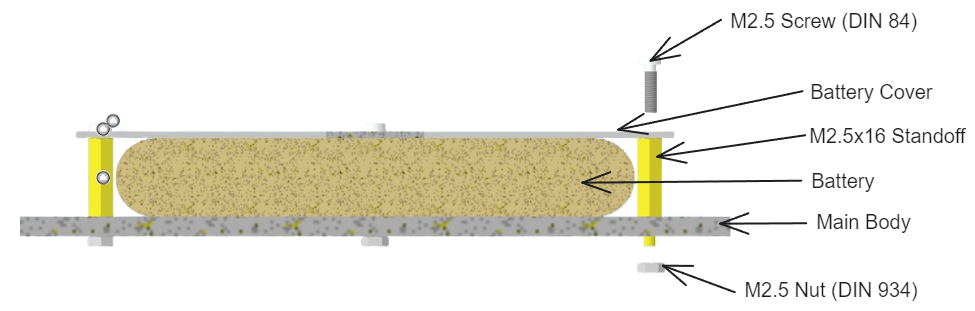
\includegraphics[height=3 cm]{texs/Part1/chapter4/image/v28.png}
        \end{minipage}
        \caption{Placement of components}
        \label{fig:variant2_battery_placement}
    \end{subfigure}
    \caption{Methods to secure the battery}
    \label{fig:variant2_battery}
\end{figure}

Solution Variant 2 employs a hybrid input method that combines both touch screen and physical buttons. The touch screen is oriented in landscape mode, while the buttons are positioned on either side of the screen (Figure \ref{fig:variant2_front_view}). To enable the integration of the touch screen, HDMI and USB connections were established between the touch screen and Raspberry Pi. Additionally, to facilitate the functionality of the physical buttons, they are connected to Raspberry Pi using general-purpose input/output  (GPIO) pins.

\begin{figure}[ht!]
    \centering
    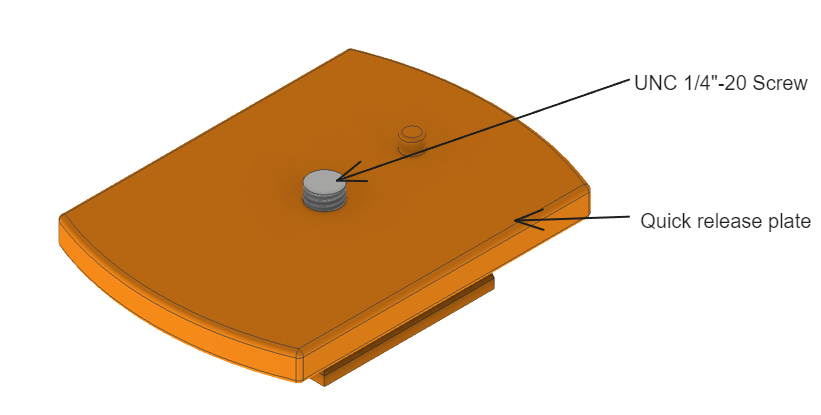
\includegraphics[height=5 cm]{texs/Part1/chapter4/image/v29.png}
    \caption{Quick release plate}
    \label{fig:variant2_quick_release_plate}
\end{figure}

In Figure \ref{fig:variant2_quick_release_plate}, we observe a quick release plate designed to be affixed to the tripod stand. To enhance stability during usage, Solution Variant 2 can utilize a quick release plate, which can be conveniently mounted on a tripod stand.

\subsubsection{Cost Calculation}
In this section, we will perform a cost analysis for producing Solution Variant 2. It is essential to emphasize that the cost calculation for the 3D printed parts solely considers the material cost and the estimated energy consumption during the printing process. Other expenses, such as the cost of the 3D printer itself, labor, and maintenance, are not factored into the calculation. Additionally, for better comparability with other variants, the costs of the Raspberry Pi, camera module, touch screen, and battery will not be included in the calculation. The formula used to calculate the cost of the 3D printed parts is as follows:

\dots


\subsection{Preliminary Design Variant 3}
\label{subsec:preliminary_design_variant_3}
Variant 3 maintains a similar component arrangement to variant 2, with the screen at the front and the camera, Raspberry Pi, and battery at the rear, as shown in Figure \ref{fig:variant3_inner_components}. However, Variant 3 introduced significant changes, such as a portrait-oriented screen and battery type.

\begin{figure}[h!]
    \centering
    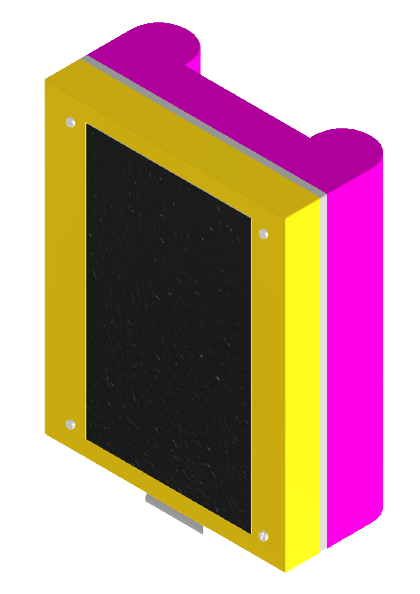
\includegraphics[height=5 cm]{texs/Part1/chapter4/image/v31.png}
    \caption{Preliminary Design Variant 3}
    \label{fig:preliminary_design_variant_3}
\end{figure}

\begin{figure}[h!]
    \centering
    \begin{subfigure}[c]{0.47\textwidth}
        \begin{minipage}{\textwidth}
            \centering
            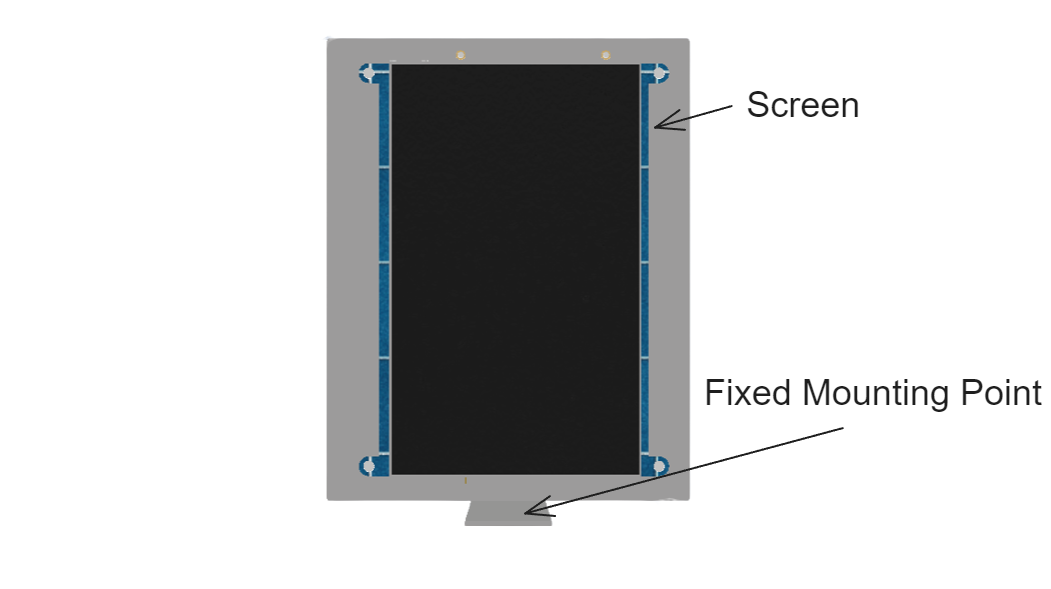
\includegraphics[height=4 cm]{texs/Part1/chapter4/image/v32.png}
        \end{minipage}
        \caption{Front View}
        \label{fig:variant3_front_components}
    \end{subfigure}
    % \hfill
    \begin{subfigure}[c]{0.5\textwidth}
        \begin{minipage}{\textwidth}
            \centering
            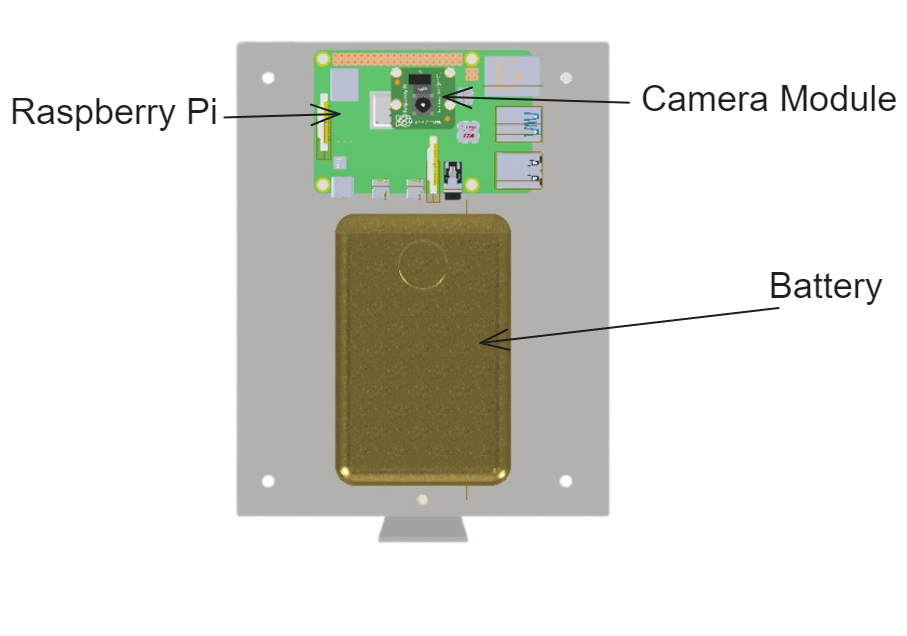
\includegraphics[height=4 cm]{texs/Part1/chapter4/image/v33.png}
        \end{minipage}
        \caption{Back View}
        \label{fig:variant3_back_components}
    \end{subfigure}
    \caption{Placement of inner components for Variant 3}
    \label{fig:variant3_inner_components}
\end{figure}

The chassis structure, similar to variant 2, comprises a main body, top cover, and back cover. The main body accommodates essential electronics and functional elements, while the top and back covers protect the internal components from external forces.

A noteworthy alteration is the inclusion of bumps on the back cover to enhance the ergonomics (Figure \ref{fig:variant3_bumps}). This adjustment aims to provide a more comfortable grip, improve user engagement, and extend the usability. In addition, the tactile bump serves as a subtle yet impactful refinement, ensuring that the device fits snugly in the user's hand, further enhancing the overall user experience. This thoughtful design element contributes to seamless and enjoyable interaction with the device.

\begin{figure}[h!]
    \centering
    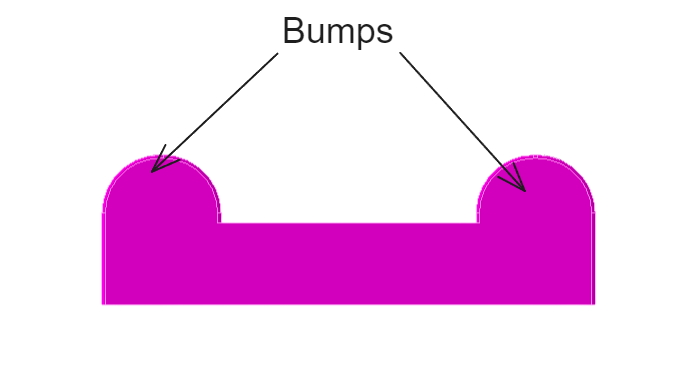
\includegraphics[width=0.5\linewidth]{texs/Part1/chapter4/image/v34.png}
    \caption{Bumps on the back cover}
    \label{fig:variant3_bumps}
\end{figure}

Variant 3 diverted from the standard battery position seen in variant 2, with a more noticeable difference in battery placement. Figure \ref{fig:variant3_battery_placement} illustrates a designated slot within the back cover, strategically designed to house a power bank outside the chassis. This configuration not only enhances the operational stability but also simplifies the process of battery replacement.

\begin{figure}[h!]
    \centering
    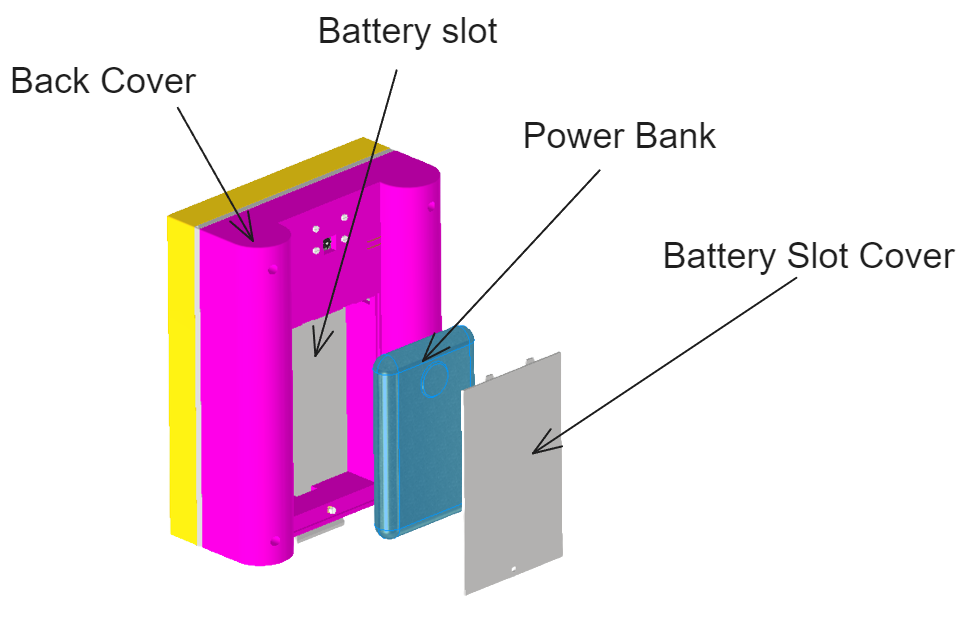
\includegraphics[width=0.5\linewidth]{texs/Part1/chapter4/image/v35.png}
    \caption{Battery Placement}
    \label{fig:variant3_battery_placement}
\end{figure}

The input methodology was streamlined using a touch screen as the sole interface. This approach simplifies the user experience by eliminating the need for physical buttons and by seamlessly integrating screen interactions. Additional information regarding the integration of the touchscreen with the Raspberry Pi is provided in the previous section.

Figure \ref{fig:variant3_front_components} also shows the integration of the mounting point of the tripod directly with the main body in Variant 3. This strategic design allows the mounting point to serve as a sturdy anchor for the device when used in a tripod stand. This direct union ensures secure and stable attachment, enhancing the versatility of the device across various usage scenarios.

\subsubsection{Cost Calculation}

\subsection{Preliminary Design Variant 6}
\label{subsec:preliminary_design_variant_6}
Figure \ref{fig:preliminary_design_variant_6} provides a detailed and comprehensive overview of the initial design concept of Variant 6. This version stands out by organizing its internal components into a configuration resembling a point-of-service (POS) system. This change from previous iterations purposefully positions the screen at an inclined angle, enhancing user interaction and optimizing the screen visibility (Figure \ref{fig:variant6_inner_components}).

\begin{figure}[h!]
    \centering
    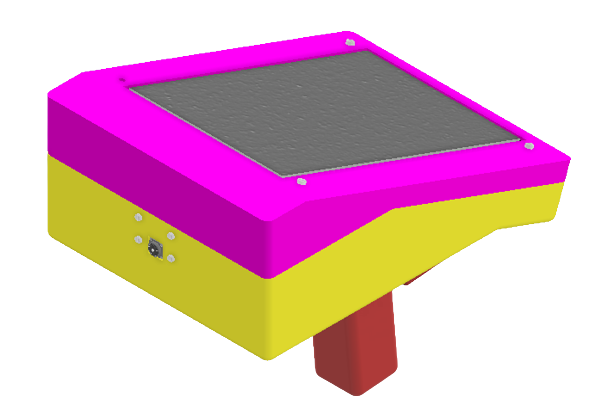
\includegraphics[height=5 cm]{texs/Part1/chapter4/image/v61.png}
    \caption{Preliminary Design Variant 6}
    \label{fig:preliminary_design_variant_6}
\end{figure}

\begin{figure}[h!]
    \centering
    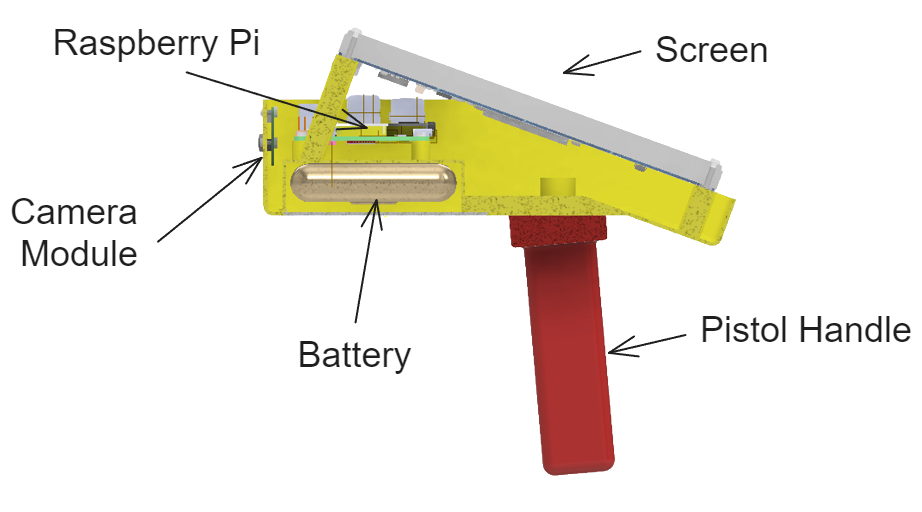
\includegraphics[height=5 cm]{texs/Part1/chapter4/image/v62.png}
    \caption{Placement of inner components for Variant 3}
    \label{fig:variant6_inner_components}
\end{figure}


Figure \ref{fig:variant6_handle_grip} demonstrates the design of the handle grip, while Figure \ref{fig:variant6_handle_grip_main_body} illustrates its placement on the main body. This ergonomic addition ensures a secure and comfortable hold during operation. Additionally, the handling of the device can be easily switched between the quick-change plate and the handle grip, providing users with flexible options for different scenarios (see Figure \ref{fig:variant6_quick_release_plate_main_body}).

\begin{figure}[h!]
    \centering
    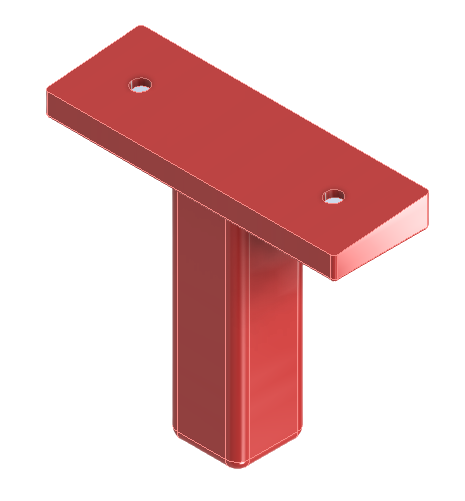
\includegraphics[width=0.5\linewidth]{texs/Part1/chapter4/image/v65.png}
    \caption{Handle Grip}
    \label{fig:variant6_handle_grip}
\end{figure}

\begin{figure}[h!]
    \centering
    \begin{subfigure}[c]{0.47\textwidth}
        \begin{minipage}{\textwidth}
            \centering
            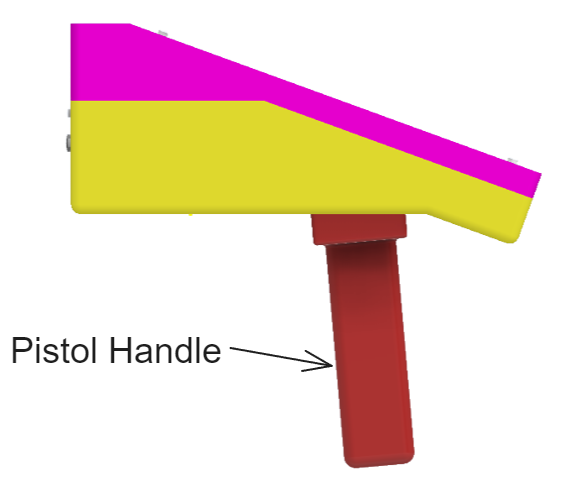
\includegraphics[height=4 cm]{texs/Part1/chapter4/image/v63.png}
        \end{minipage}
        \caption{Handle Grip with Main Body}
        \label{fig:variant6_handle_grip_main_body}
    \end{subfigure}
    % \hfill
    \begin{subfigure}[c]{0.5\textwidth}
        \begin{minipage}{\textwidth}
            \centering
            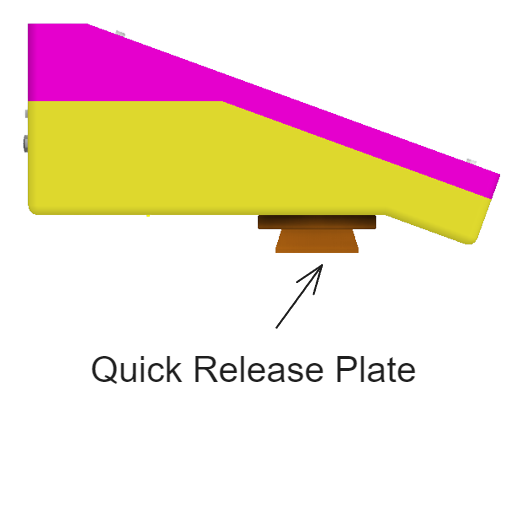
\includegraphics[height=4 cm]{texs/Part1/chapter4/image/v64.png}
        \end{minipage}
        \caption{Quick Release Plate with Main Body}
        \label{fig:variant6_quick_release_plate_main_body}
    \end{subfigure}
    \caption{Placement of handle grip and quick release plate}
    \label{fig:variant6_handle_grip_quick_release_plate}
\end{figure}


This variant boasts the same input method and battery placement as Variant 3. For a comprehensive explanation regarding these aspects, please refer to Section \ref{subsec:preliminary_design_variant_3}. Touch screens serve as the primary input modality, providing an intuitive and seamless interaction experience. Furthermore, the battery is tucked away in a slot on the back cover and is secured by screws and threaded inserts.

\subsubsection{Cost Calculation}


\subsection{Preliminary Design Variant 7}
Figure \ref{fig:preliminary_design_variant_7} shows the intriguing concept of variant 7, which is influenced by the handheld PC approach. Here, Raspberry Pi cleverly integrates with the back of the screen, forming a compact and unified structure. Simultaneously, the battery aligned gracefully beside the screen, creating a harmonious arrangement.

\begin{figure}[h!]
    \centering
    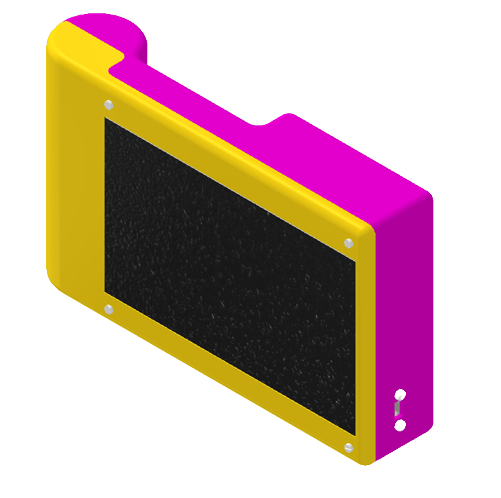
\includegraphics[height=5 cm]{texs/Part1/chapter4/image/v71.png}
    \caption{Preliminary Design Variant 7}
    \label{fig:preliminary_design_variant_7}
\end{figure}

\begin{figure}[h!]
    \centering
    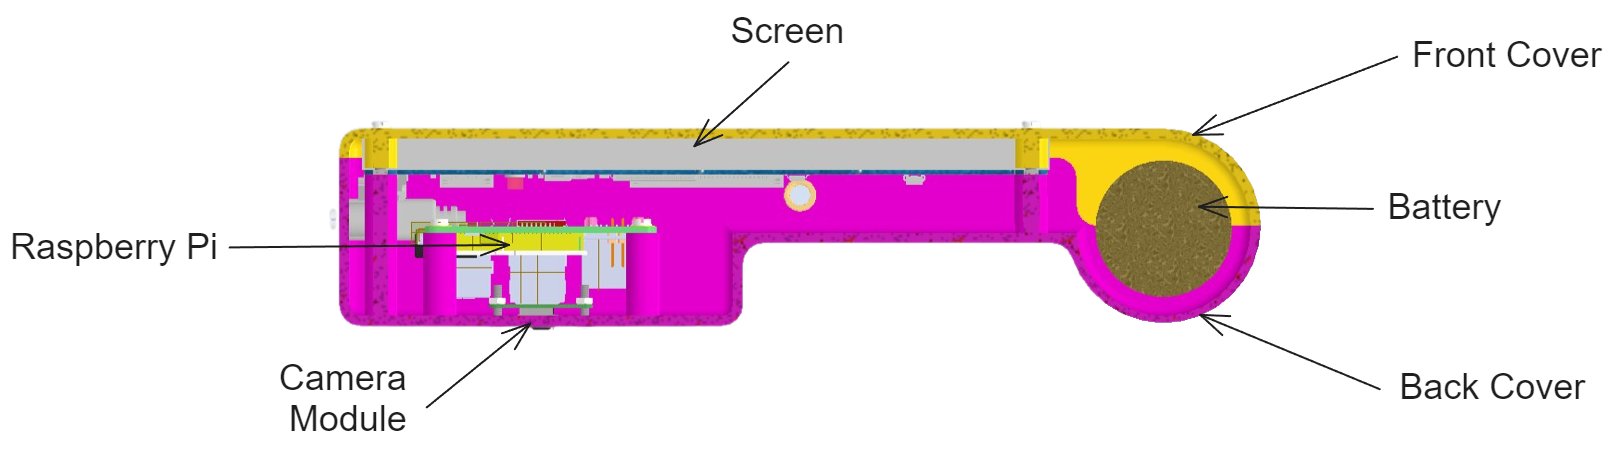
\includegraphics[height=3 cm]{texs/Part1/chapter4/image/v72.png}
    \caption{Placement of inner components for Variant 7}
    \label{fig:variant7_inner_components}
\end{figure}

The device features a strategically placed bump on the side, which improves ergonomics and serves as a secure enclosure for the battery (Figure \ref{fig:variant7_inner_components}). The control methods in this variant were similar to those in variant 2, utilizing only touch interfaces.

\begin{figure}[h!]
    \centering
    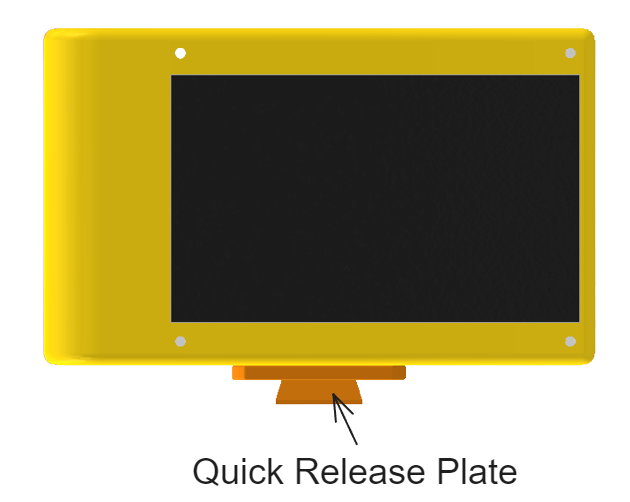
\includegraphics[height=5 cm]{texs/Part1/chapter4/image/v73.png}
    \caption{Placement of quick release plate}
    \label{fig:variant7_quick_release_plate}
\end{figure}

Similar to variants 2 and 6, this variant also utilized the quick release plate to enable integration with a tripod stand. The placement of the plate can be seen in Figure \ref{fig:variant7_quick_release_plate}.



\subsubsection{Cost Calculation}

\section{Evaluation with VDI 2225}
In this section, we will evaluate the preliminary design variants by utiliting the guideline VDI 2225 \cite{Pahl07ac}. This guideline is a comprehensive framework for evaluating technical solutions based on a balanced consideration of various aspects.

To achieve this, the guideline advocates for methods that provide a holistic evaluation, covering both task-specific requirements and general constraints. These methods aim to not only quantify but also qualitatively assess the properties of different variants, even in the early conceptual phase where information is limited.

The evaluation process, as discussed by Pahl and Beitz \cite{Pahl07ac}, outlined in the guideline involves several key steps:

\subsubsection{Identifying Evaluation Criteria}
This initial step involves defining a set of objectives from which specific evaluation criteria can be derived. These objectives should comprehensively cover decision-relevant requirements and general constraints, ensuring that no crucial criteria are overlooked. The objectives should also be as independent of each other as possible, and expressed in either quantitative or qualitative terms.

Followings are the evaluation criteria for the preliminary design variants:

\textbf{Weight Distribution:} The weight distribution is evaluated based on the weight distribution of the variants and the weight distribution of the individual components. The value for weight distribution is retrieved from Computer-Aided Design (CAD) models through detailed analysis of the device's structural layout and component placement.

\textbf{Device Weight:} Device weight evaluates the overall heaviness of the equipment. A lighter device is generally easier to handle and transport, reducing user fatigue and enabling greater mobility while maintaining performance and durability. The value for device weight is calculated from Computer-Aided Design (CAD) models by summing the individual weights of all components, materials, and structural elements that constitute the device.

\textbf{Device Size:} The size criterion considers the physical dimensions of the device, assessing its compactness and portability. An optimal device size allows for convenient storage, transportation, and operation in various environments without compromising functionality. The evaluation of device size involves measuring key dimensions such as length, width, height, and any protrusions or extensions.

\textbf{Ease of Assembly:} This criterion evaluates the ease of assembling and disassembling the device. Quick and easy assembly and disassembly saves time and increases user convenience, reducing the risk of errors. Evaluation is done by counting the components used in assembly and disassembly. Fewer components often mean a simpler and more user-friendly design. The type and number of fasteners, such as screws or connectors, needed for assembly are also considered.

\textbf{Swappable Parts:} Swappable components refer to the ease with which parts can be interchanged or substituted. This design enhances flexibility, maintenance, and adaptability. The presence of swappable parts encourages component modularity, enabling streamlined repairs and upgrades. Assessment of swappable parts is based on the quantity of interchangeable components and their compatibility. A higher number of swappable parts signifies a design that supports versatility and minimizes downtime for maintenance or repairs.

\subsubsection{Weighting Evaluation Criteria}
After establishing the evaluation criteria, their relative importance is assessed through weighting factors, $w$. This step is crucial in eliminating less significant criteria before the actual evaluation. Weightings should reflect the relative importance of each evaluation criterion.

Guideline VDI 2225 aims to avoid weightings and instead relies on criteria of roughly equal importance. However, weightings (like 2x or 3x) are used when there are significant differences between criteria.
Table \ref{tab:weighting} shows the weighting factors for the evaluation criteria.

\begin{table}[!h]
    \centering
    \begin{tabular}{|l|c|}
        \hline
        \textbf{Criteria}   & \textbf{Weighting Factor, $w$} \\ \hline
        Weight Distribution & 2x                             \\ \hline
        Device Weight       & 3x                             \\ \hline
        Device Size         & 1x                             \\ \hline
        Ease of Assembly    & 1x                             \\ \hline
        Swappable Parts     & 1x                             \\ \hline
    \end{tabular}
    \caption{Weighting Factors for Evaluation Criteria}
    \label{tab:weighting}
\end{table}

\subsubsection{Assessing Values}
This step involves assigning values, $v_{ij}$, to the variants based on the relative scale of the determined parameters. Guideline VDI 2225 suggests using a range from 0 to 4 for this purpose. Table \ref{tab:value_scale} shows the scale used for the evaluation of the preliminary design variants. \Cref{tab:value_scale_weight_distribution,tab:value_scale_device_weight,tab:value_scale_device_size,tab:value_scale_ease_of_assembly,tab:value_scale_swappable_parts} show the value scales for the individual evaluation criteria. Equation \ref{eq:weight_calculation} shows the formula used to calculate the weighted value, $wv_{ij}$, for each variant.

\begin{table}[!h]
    \centering
    \begin{tabular}{|c|c|}
        \hline
        \textbf{Points, $v_{ij}$} & \textbf{Meaning}  \\ \hline
        0                         & unsatisfactory    \\ \hline
        1                         & just tolerable    \\ \hline
        2                         & adequate          \\ \hline
        3                         & good              \\ \hline
        4                         & very good (ideal) \\ \hline
    \end{tabular}
    \caption{Value Scale for Evaluation \cite{Pahl07ad}}
    \label{tab:value_scale}
\end{table}

\begin{table}[H]
    \centering
    \begin{tabular}{|c|c|}
        \hline
        \multicolumn{2}{|c|}{\textbf{Weight Distribution}} \\ \hline
        \textbf{Range, mm} & \textbf{Point, $v_{ij}$}      \\ \hline
        0-10               & 4                             \\ \hline
        10-50              & 3                             \\ \hline
        50-100             & 2                             \\ \hline
        100-150            & 1                             \\ \hline
        $\geq$ 150         & 0                             \\ \hline
    \end{tabular}
    \caption{Value Scale for Weight Distribution}
    \label{tab:value_scale_weight_distribution}
\end{table}

\begin{table}[H]
    \centering
    \begin{tabular}{|c|c|}
        \hline
        \multicolumn{2}{|c|}{\textbf{Device Weight}} \\ \hline
        \textbf{Range, g} & \textbf{Point, $v_{ij}$} \\ \hline
        0-500             & 4                        \\ \hline
        500-1000          & 3                        \\ \hline
        1000-1500         & 2                        \\ \hline
        1500-2000         & 1                        \\ \hline
        $\geq$ 2000       & 0                        \\ \hline
    \end{tabular}
    \caption{Value Scale for Device Weight}
    \label{tab:value_scale_device_weight}
\end{table}

\begin{table}[H]
    \centering
    \begin{tabular}{|c|c|}
        \hline
        \multicolumn{2}{|c|}{\textbf{Device Size}}    \\ \hline
        \textbf{Range, mm} & \textbf{Point, $v_{ij}$} \\ \hline
        0-100              & 4                        \\ \hline
        100-200            & 3                        \\ \hline
        200-300            & 2                        \\ \hline
        300-400            & 1                        \\ \hline
        $\geq$ 400         & 0                        \\ \hline
    \end{tabular}
    \caption{Value Scale for Device Size}
    \label{tab:value_scale_device_size}
\end{table}

\begin{table}[H]
    \centering
    \begin{tabular}{|c|c|}
        \hline
        \multicolumn{2}{|c|}{\textbf{Ease of Assembly}} \\ \hline
        \textbf{Range} & \textbf{Point, $v_{ij}$}       \\ \hline
        0-25           & 4                              \\ \hline
        25-50          & 3                              \\ \hline
        50-75          & 2                              \\ \hline
        75-100         & 1                              \\ \hline
        $\geq$ 100     & 0                              \\ \hline
    \end{tabular}
    \caption{Value Scale for Ease of Assembly}
    \label{tab:value_scale_ease_of_assembly}
\end{table}

\begin{table}[H]
    \centering
    \begin{tabular}{|c|c|}
        \hline
        \multicolumn{2}{|c|}{\textbf{Swappable Parts}} \\ \hline
        \textbf{Range} & \textbf{Point, $v_{ij}$}      \\ \hline
        $\geq$ 4       & 4                             \\ \hline
        3              & 3                             \\ \hline
        2              & 2                             \\ \hline
        1              & 1                             \\ \hline
        0              & 0                             \\ \hline
    \end{tabular}
    \caption{Value Scale for Swappable Parts}
    \label{tab:value_scale_swappable_parts}
\end{table}

\begin{equation}
    wv_{ij} = w_{i} \cdot v_{ij}
    \label{eq:weight_calculation}
\end{equation}


\subsubsection{Determining the Overall Value}
The overall value of each variant, $OWV_{j}$, is calculated by summing the weighted values, $wv_{ij}$, of all evaluation criteria (see Equation \ref{eq:weighted_sum}).

\begin{equation}
    OWV_{j}=\sum_{i=1}^{n}wv_{ij}
    \label{eq:weighted_sum}
\end{equation}

\subsubsection{Comparing Concept Variants}
With the overall values, $OWV_{j}$, of the concept variants, the variants can be compared and evaluated based on thier rating, $R$, which is calculated using Equation \ref{eq:total_rating}. The technical rating, $R_{t}$, is calculated using Equation \ref{eq:technical_rating}, where $v_{max}$ is the maximum value of the value scale, and $n$ is the number of evaluation criteria.

The economic rating, $R_{e}$, is calculated using Equation \ref{eq:economic_rating}, where $C_{o}$ is the comparative cost, and $C_{variant}$ is the cost of the variant. For this project, the comparative cost, $C_{o}$, is set to be 60\% of the cost of the least expensive variant (see Equation \ref{eq:comparative_cost}).

The best variant is determined by comparing the total rating, $R$, of each variant. The variant with the highest total rating is considered the best variant.

\begin{equation}
    R=\frac{R_{t}+R_{e}}{2}
    \label{eq:total_rating}
\end{equation}

\begin{equation}
    R=\frac{OWV_{j}}{v_{max}\cdot\sum_{i=1}^{n}w_{i}}
    \label{eq:technical_rating}
\end{equation}

\begin{equation}
    R=\frac{C_{o}}{C_{variant}}
    \label{eq:economic_rating}
\end{equation}

\begin{equation}
    C_{o}=0.6\cdot C_{minimum}
    \label{eq:comparative_cost}
\end{equation}

\subsection{Evaluation of Preliminary Design Variant}
In this section, the result of the evaluation of the preliminary design variants will be presented. Table \ref{tab:tech_eval} shows the technical evaluation of the preliminary design variants, while Table \ref{tab:economic_eval} shows the economic evaluation of the variants. The total rating of the variants is shown in Table \ref{tab:total_rating}. Based on the total rating, Variant 6 is the best variant, followed by Variant 7, Variant 3, and Variant 2.

For a more detailed calculation, please refer to Appendix \ref{appendix:technical_evaluation}.


\begin{table}[h]
    \centering
    \begin{tabular}{|c|c|c|}
        \hline
        \multicolumn{3}{|c|}{\textbf{Production Cost}}                                                 \\ \hline
        \textbf{Variant} & \textbf{Cost, $C_{variant}$(\texteuro)} & \textbf{Economic Rating, $R_{e}$} \\ \hline
        Variant 2        & 74.95                                   & 0.33                              \\ \hline
        Variant 3        & 47.97                                   & 0.52                              \\ \hline
        Variant 6        & 44.14                                   & 0.56                              \\ \hline
        Variant 7        & 41.25                                   & 0.60                              \\ \hline
    \end{tabular}
    \caption{Economic Evaluation of Preliminary Design Variants}
    \label{tab:economic_eval}
\end{table}

\begin{table}[!h]
    \centering
    \begin{tabular}{|c|c|c|c|}
        \hline
        \textbf{Variant} & \textbf{Technical Rating, $R_{t}$} & \textbf{Economic Rating, $R_{e}$} & \textbf{Total Rating, $R$} \\ \hline
        Variant 2        & 0.65                               & 0.33                              & 0.4901                     \\ \hline
        Variant 3        & 0.60                               & 0.52                              & 0.5580                     \\ \hline
        Variant 6        & 0.70                               & 0.56                              & 0.6304                     \\ \hline
        Variant 7        & 0.65                               & 0.60                              & 0.6250                     \\ \hline
    \end{tabular}
    \caption{Total Rating of Preliminary Design Variants}
    \label{tab:total_rating}
\end{table}

\begin{table}[H]
    \centering
    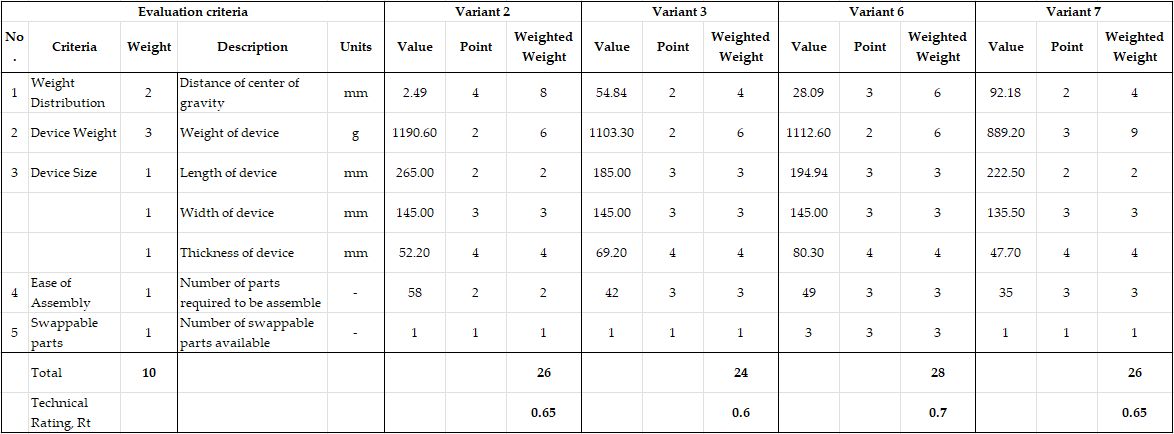
\includegraphics[angle=90,origin=c, width=0.5\linewidth]{texs/Part1/chapter4/image/tech_eval.png}
    \caption{Technical Evaluation of Preliminary Design Variants}
    \label{tab:tech_eval}
\end{table}

\section{Detail Design}
\label{sec:detail_design}
The result of the evaluation of the preliminary design variants shows that Variant 6 is the best variant. Hence, this variant will be used as the basis for the detail design. Any improvements will be added in the design, while any weaknesses will be addressed. The result of this process is the final design of the device.

\subsubsection{Power Switch}

This component plays a critical role in controlling the Raspberry Pi's power supply. It is imperative to have a reliable method for powering up and shutting down the Raspberry Pi to ensure smooth operation and prevent potential data corruption.

One available method utilizes the GPIO (General Purpose Input/Output) pins to initiate a shutdown sequence for the Raspberry Pi \cite{Labidi21}. While effective in bringing the device to a hibernation state, it's important to note that this method doesn't completely cut off power. As a result, the Raspberry Pi still draws a minimal amount of power even in this low-power state \cite{jdb}.

To achieve more efficient power management, a more straightforward approach is recommended. This involves the implementation of a simple physical switch (refer to Figure \ref{}). This switch functions by directly connecting and disconnecting the power supply to the Raspberry Pi. As a result, when the switch is in the "off" position, it completely severs the power supply, ensuring that the Raspberry Pi consumes no power whatsoever. This approach has been chosen as the preferred method for controlling the power supply in this project due to its effectiveness and simplicity in implementation.

\subsubsection{Camera Protection}

In the context of the device's design considerations, particular attention has been directed towards safeguarding the camera component. As illustrated in Figure \ref{fig:camera_position}, the current design accommodates the camera within the body of the device, with the lens extending slightly beyond its confines.

\begin{figure}[h!]
    \centering
    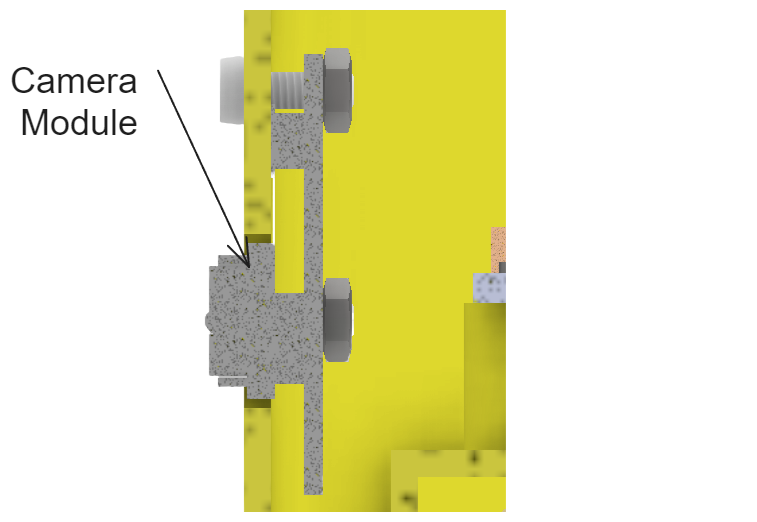
\includegraphics[height=5 cm]{texs/Part1/chapter4/image/d1.png}
    \caption{Position of the camera component}
    \label{fig:camera_position}
\end{figure}

While this configuration is essential for optimal functionality, it does pose a potential vulnerability. Specifically, there exists a risk of inadvertent damage to the camera lens if the device is mistakenly positioned with the lens side facing a surface. Such damage, if incurred, could have severe repercussions on the device's usability.

To address this concern, a purposeful addition has been made in the form of a 3 mm high protective bump (see Figure \ref{fig:detail_camera_protect}). Strategically placed, this bump serves as a safeguard, effectively elevating the camera lens above surfaces and thus averting direct contact.

\begin{figure}[h!]
    \centering
    \begin{subfigure}[c]{0.47\textwidth}
        \begin{minipage}{\textwidth}
            \centering
            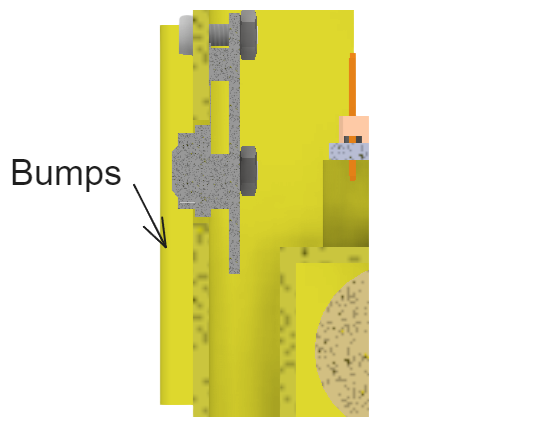
\includegraphics[height=4 cm]{texs/Part1/chapter4/image/d12.png}
        \end{minipage}
        \caption{Left View}
        \label{fig:detail_camera_left}
    \end{subfigure}
    \begin{subfigure}[c]{\textwidth}
        \begin{minipage}{\textwidth}
            \centering
            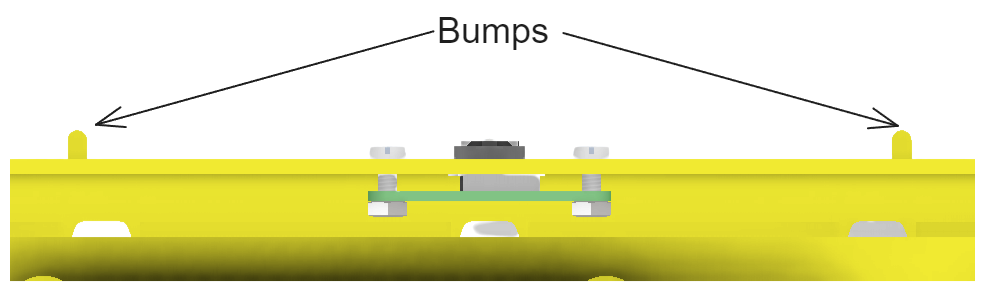
\includegraphics[width=0.75\linewidth]{texs/Part1/chapter4/image/d13.png}
        \end{minipage}
        \caption{Top View}
        \label{fig:detail_camera_top}
    \end{subfigure}
    \caption{Protective bump for camera}
    \label{fig:detail_camera_protect}
\end{figure}

\subsubsection{Screen Protection}
In parallel to the considerations for camera protection, an analogous concern extends to safeguarding the device's screen. The design, as depicted in Figure, accommodates a screen that sits flush with the device's surface, rendering it susceptible to potential damage if placed on abrasive or uneven surfaces.

Similar to the implementation for camera protection, a parallel measure has been applied to address concerns regarding screen protection. As depicted in Figure \ref{fig:detail_screen_protect}, the design integrates a protective bump around the screen perimeter, mirroring the approach taken for the camera.

\begin{figure}[h!]
    \centering
    \begin{subfigure}[c]{0.47\textwidth}
        \begin{minipage}{\textwidth}
            \centering
            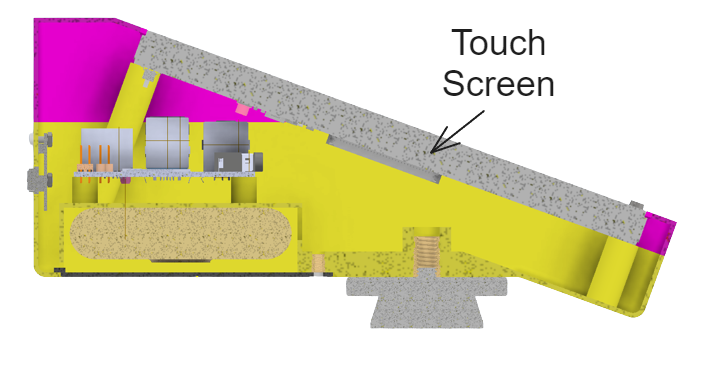
\includegraphics[height=3.5 cm]{texs/Part1/chapter4/image/d21.png}
        \end{minipage}
        \caption{Before}
        \label{fig:detail_screen_before}
    \end{subfigure}
    \begin{subfigure}[c]{0.47\textwidth}
        \begin{minipage}{\textwidth}
            \centering
            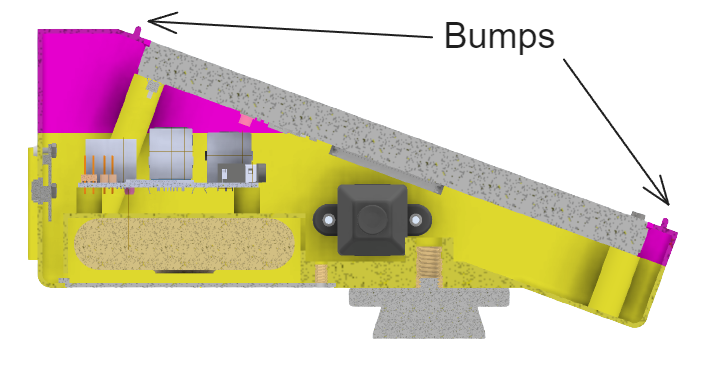
\includegraphics[height=3.5 cm]{texs/Part1/chapter4/image/d22.png}
        \end{minipage}
        \caption{After}
        \label{fig:detail_screen_after}
    \end{subfigure}
    \caption{Protective bump for screen}
    \label{fig:detail_screen_protect}
\end{figure}

\subsubsection{Column for Threaded Inserts}
In accordance with the design specifications detailed in section \ref{}, threaded inserts have been employed as a critical element for securely fastening components within the body of the device.

It is imperative to note that threaded inserts of varying sizes necessitate distinct minimum wall thicknesses for the columns, as well as specific hole depths to ensure proper engagement and stability. To address this requirement, a comprehensive sizing guide based on Ruthex threaded inserts has been compiled and is presented in Table \ref{tab:threaded_inserts_sizing_guide}.

\begin{table}[!h]
    \centering
    \begin{tabular}{|c|c|c|c|}
        \hline
        \textbf{Thread Size} & \textbf{Hole size (mm)} & \textbf{Min. thickness (mm)} & \textbf{Min. height (mm)} \\ \hline
        M2.5                 & 4                       & 1.6                          & 6.7                       \\ \hline
        1/4"                 & 8                       & 3.3                          & 13.7                      \\ \hline
    \end{tabular}
    \caption{Sizing guide for threaded inserts \cite{ruthex1}\cite{ruthex2}}
    \label{tab:threaded_inserts_sizing_guide}
\end{table}


\subsubsection{LAN Port}

The inclusion of a LAN (Local Area Network) port in the device design serves as a crucial convenience feature for users seeking to perform maintenance on the Raspberry Pi without the need for disassembly. This strategic integration allows for seamless connectivity, enabling direct access to the Raspberry Pi's functionalities and resources over a local network. Figure \ref{fig:lan_port} shows the LAN port.

Positioned on the side of the device body (see Figure \ref{fig:lan_port_position}), the LAN port offers a user-friendly interface, ensuring easy accessibility for maintenance tasks. This thoughtful placement not only enhances the overall user experience but also demonstrates a commitment to user-centric design, allowing for swift and efficient maintenance procedures while minimizing any potential disruption to the device's internal components.

\begin{figure}[h!]
    \centering
    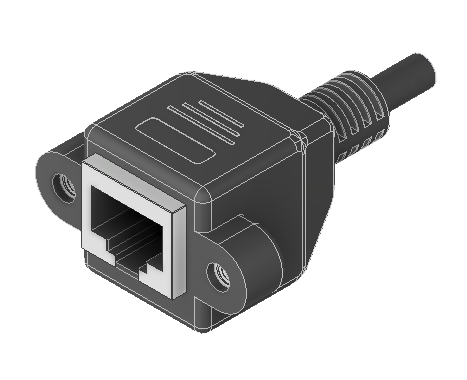
\includegraphics[height=5 cm]{texs/Part1/chapter4/image/d31.png}
    \caption{The LAN port}
    \label{fig:lan_port}
\end{figure}

\begin{figure}[h!]
    \centering
    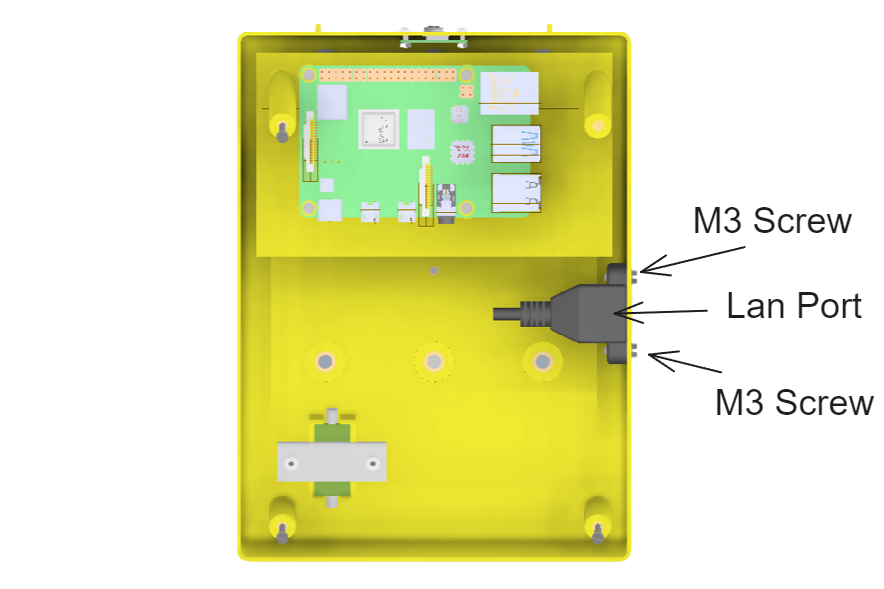
\includegraphics[height=5 cm]{texs/Part1/chapter4/image/d32.png}
    \caption{Position of the LAN port}
    \label{fig:lan_port_position}
\end{figure}

\subsubsection{Color Scheme}

The color scheme plays a crucial role in enhancing the product's appeal. Considering the target market is the police force, we drew inspiration from the Germany police logo, as can be seen in Figure \ref{fig:polizei_logo}. Blue, the dominant color in the logo, is used as the primary color for the device. Other color that is presented in the logo is yellow, which is used as the device's handle grip color and the color white, which is used as the color for the devices top cover.

The result of the color scheme can be seen in Figure \ref{fig:color_scheme}.

\begin{figure}[h!]
    \centering
    
\includegraphics[height=5 cm]{texs/Part1/chapter4/image/polizei.jpg}
    \caption{Germany Police Logo \cite{bundespolizei}}
    \label{fig:polizei_logo}
\end{figure}

\begin{figure}[h!]
    \centering
    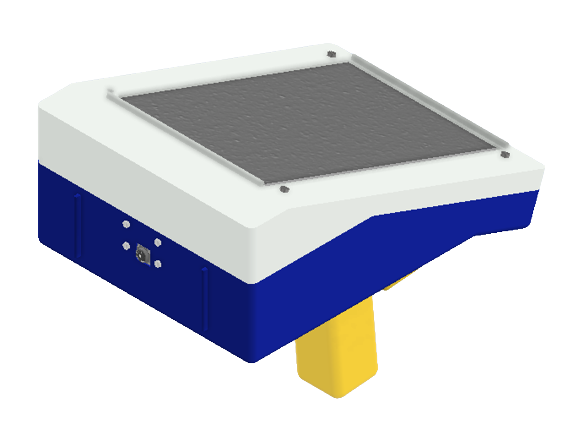
\includegraphics[height=9 cm]{texs/Part1/chapter4/image/d41.png}
    \caption{Result of recolor}
    \label{fig:color_scheme}
\end{figure}


